\documentclass[11pt,a4paper]{article}

\usepackage[margin=1in]{geometry}
\usepackage{amsmath}
\usepackage{tikz}
\usepackage{float}
\usepackage{parskip}
\usepackage{adjustbox}

\usetikzlibrary{positioning, arrows.meta}

\title{Graph Data Collection and Construction}
\author{Ryan Pek}
\date{\today}

\begin{document}

\maketitle

\section{Overview}

The Singapore bus network is modelled as a directed graph:

\[
G = (V, E)
\]

where:

\begin{itemize}
    \item $V$ is the set of bus stops
    \item $E \subseteq V \times V$ is the set of valid directed transitions
\end{itemize}

An edge $(u,v)$ exists if there exists a bus service $s$ and direction $d$ such that $v$ is the immediate successor of $u$ in the ordered route sequence of $(s,d)$.

The objective of this stage is to construct $G$ from raw LTA DataMall data.

\section{Data Sources}

The following endpoints are used:

\begin{itemize}
    \item \textbf{BusStops}: metadata (stop code, description, coordinates)
    \item \textbf{BusRoutes}: ordered stop sequences for each service
    \item \textbf{BusServices}: service-level metadata
    \item \textbf{BusArrival}: used to determine service presence at stops
\end{itemize}

All responses are stored as raw JSON snapshots without modification.

\subsection{Pagination and Empirical Limits}

All endpoints return data in pages of up to 500 records, accessed via:

\[
\texttt{?\$skip=} n \cdot 500
\]

where $n$ is the page index.

Empirically observed payload counts (as of last collection):

\begin{itemize}
    \item \textbf{BusStops}: $\approx 11$ pages
    \item \textbf{BusRoutes}: $\approx 51$ pages
    \item \textbf{BusServices}: $\approx 2$ pages
\end{itemize}

In implementation, one additional page is queried beyond these values to detect changes in dataset size.

These values are not assumed fixed and should be treated as lower bounds.

\section{Data Pipeline}

\begin{figure}[H]
\centering
\begin{adjustbox}{max width=\textwidth}
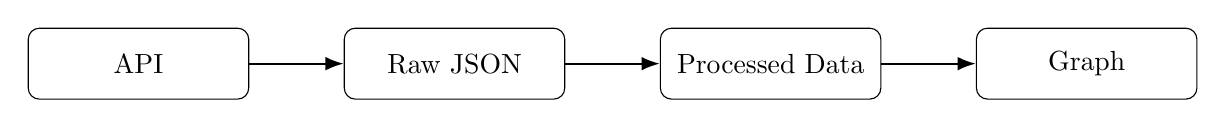
\begin{tikzpicture}[
    node distance=1.2cm,
    box/.style={
        draw,
        rounded corners,
        minimum width=2.8cm,
        minimum height=0.9cm,
        align=center
    },
    arrow/.style={-Latex, thick}
]

\node[box] (api) {API};
\node[box, right=of api] (raw) {Raw JSON};
\node[box, right=of raw] (proc) {Processed Data};
\node[box, right=of proc] (graph) {Graph};

\draw[arrow] (api) -- (raw);
\draw[arrow] (raw) -- (proc);
\draw[arrow] (proc) -- (graph);

\end{tikzpicture}
\end{adjustbox}
\caption{Data flow}
\end{figure}

\section{Construction}

\subsection{Vertex Set}

The vertex set is constructed as:

\begin{itemize}
    \item union of all \texttt{BusStopCode} from BusStops
    \item union of all \texttt{BusStopCode} from BusRoutes
    \item deduplicated
\end{itemize}

This ensures coverage in the presence of incomplete or inconsistent datasets.

\subsection{Route Extraction}

For each service:

\begin{itemize}
    \item group entries by \texttt{ServiceNo}
    \item split by \texttt{Direction}
    \item entries are sorted by \texttt{StopSequence} to recover traversal order
\end{itemize}

Each service produces up to two ordered sequences:

\[
R_{s,1}, \quad R_{s,2}
\]

\subsection{Edge Construction}

Given a route:

\[
R = [v_1, v_2, \dots, v_k]
\]

edges are constructed as:

\[
(v_1,v_2), (v_2,v_3), \dots, (v_{k-1},v_k)
\]

The final edge set is the union over all services and directions.

Duplicate edges are collapsed into a single adjacency entry.

\subsection{Adjacency Representation}

The graph is stored as an adjacency map:

\begin{verbatim}
{
  "85049": {
    "neighbours": [...],
    "distfromint": ...,
    "timesvisited": 0
  }
}
\end{verbatim}

\subsection{Node Fields}

\begin{itemize}
    \item \texttt{neighbours}: outgoing edges
    \item \texttt{distfromint}: distance from route origin
    \item \texttt{timesvisited}: mutable traversal metadata used by search algorithms
\end{itemize}

\section{Properties}

\begin{itemize}
    \item directed graph
    \item contains cycles (loop services)
    \item not guaranteed strongly connected
    \item multiple services may induce identical edges
\end{itemize}

\section{Edge Cases}

\subsection{Terminal Stops}

Final stops in a route have no outgoing edges.

\subsection{Loop Services}

Loop services (e.g. 225G / 225W):

\begin{itemize}
    \item form cycles
    \item must be treated as separate directed paths
\end{itemize}

\subsection{Self-loops}

Certain stops may incorrectly reference themselves as neighbours due to data anomalies.

These are explicitly filtered during graph construction.

\subsection{Data Inconsistencies}

Observed issues:

\begin{itemize}
    \item stops present in routes but missing from stops dataset
    \item services appearing in arrival data but not in route data
    \item occasional malformed neighbour relationships
\end{itemize}

These are handled manually or filtered during processing.

\section{Implementation Notes}

The system is implemented in two stages:

\begin{itemize}
    \item Python prototype:
    \begin{itemize}
        \item data collection
        \item graph construction
    \end{itemize}

    \item Go rewrite:
    \begin{itemize}
        \item API layer (HTTP fetch)
        \item storage layer (JSON + filesystem)
        \item graph construction layer
    \end{itemize}
\end{itemize}

\end{document}
